
\documentclass{Bredelebeamer}
\usepackage{anyfontsize}
\usepackage{hyperref}


%%%%%%%%%%%%%%%%%%%%%%%%%%%%%%%%%%%%%%%%%%%%%%%%



\title[\textbf{Presentazione AISF}]{
\includegraphics[scale=2]{images/aisf.png} \\Presentazione Associazione Italiana Studenti di Fisica}
% Titolo della presentazione

\subtitle{\textbf{ Matter of Physics}}
% Sottotitolo opzionale

\author{Marco Morrone \inst{}}
% La commande \inst{...} Permet d'afficher l' affiliation de l'intervenant.
% Si il y a plusieurs intervenants: Marcel Dupont\inst{1}, Roger Durand\inst{2}
% Il suffit alors d'ajouter un autre institut sur le modèle ci-dessous.

\institute[Ass. Italiana Studenti di Fisica]
{
  \inst{}%
 {\footnotesize Event Coordinator \\ \textit{ marco.morrone@ai-sf.it}}
  }

\date{17 maggio 2016}
% Optionnel. La date, généralement celle du jour de la conférence

\subject{Presentazione AISF}
% C'est utilisé dans les métadonnes du PDF



\logo{

\includegraphics[scale=0.6]{images/aisf.png}
}



%%%%%%%%%%%%%%%%%%%%%%%%%%%%%%%%%%%%%%%%%%%%%%%%%%%%%%%%%%%%%%%%%%%%%
\begin{document}

\begin{frame}
  \titlepage
\end{frame}

\section{Chi Siamo}

\begin{frame}
\begin{block}{\centering{\fontsize{30}{100}\selectfont CHI SIAMO}}
\end{block}
\end{frame} 
\subsection{Introduzione}
\begin{frame}{Chi Siamo}
L'\thinspace Associazione Italiana Studenti di Fisica (AISF) è un'organizzazione con finalità educative e senza fine di lucro che ambisce a riunire tutti gli studenti di Fisica d'Italia.
\begin{figure}
\begin{block}{\centering \textbf{Tappe Costituenti}}
\begin{itemize}
\item 15 Agosto 2014 - ICPS @ Heidelberg  [14]
\item 15-17 Maggio 2015 - CISF @ Torino [130]
\item 16 Agosto 2015 - ICPS @ Zagreb [160]
\item 22-24 Aprile 2016 - CISF @ Torino [430]
\end{itemize}
\end{block}
\begin{block}{\centering \textbf{Perché AISF}}
\begin{itemize}
\item AISF è National Committee dell'International Association of Physics Students
\item Network di studenti italiani e stranieri
\item Organizzazione eventi scientifici nei centri di ricerca
\item Organizzazione eventi divulgativi
\end{itemize}
\end{block}
\end{figure}
\end{frame}
\subsection{CLEEC}
\begin{frame}{Comitato Esecutivo}
\begin{figure}
\begin{block}{\centering \textbf{Membri Comitato Esecutivo}}
\begin{itemize}
\item \textbf{Presidente}: Andrea Celon (Valerio Peri)
\item \textbf{VicePresidente}: Marta Crisanti
\item \textbf{Tesoriere}: Michele Re Fiorentin
\item \textbf{Segretario}: Vittorio Erba
\item \textbf{Relazioni Esterne e con Comitati Locali}: Marta Crisanti (Marianna d'Amato)
\item \textbf{Coordinatore Eventi}: Francesco Sciortino (Marco Morrone)
\item \textbf{IT Manager e Affari Esteri}: Giulio Pasqualetti (Gabriele di Ubaldo)
\item \textbf{Responsabile Progetto FERMI}: Lucio Maria Milanese
\end{itemize}
\end{block}
\end{figure}
\end{frame}
\section{Provenienza Geografica}
\subsection{Mappa}
\begin{frame}{Provenienza Geografica}
\begin{figure}
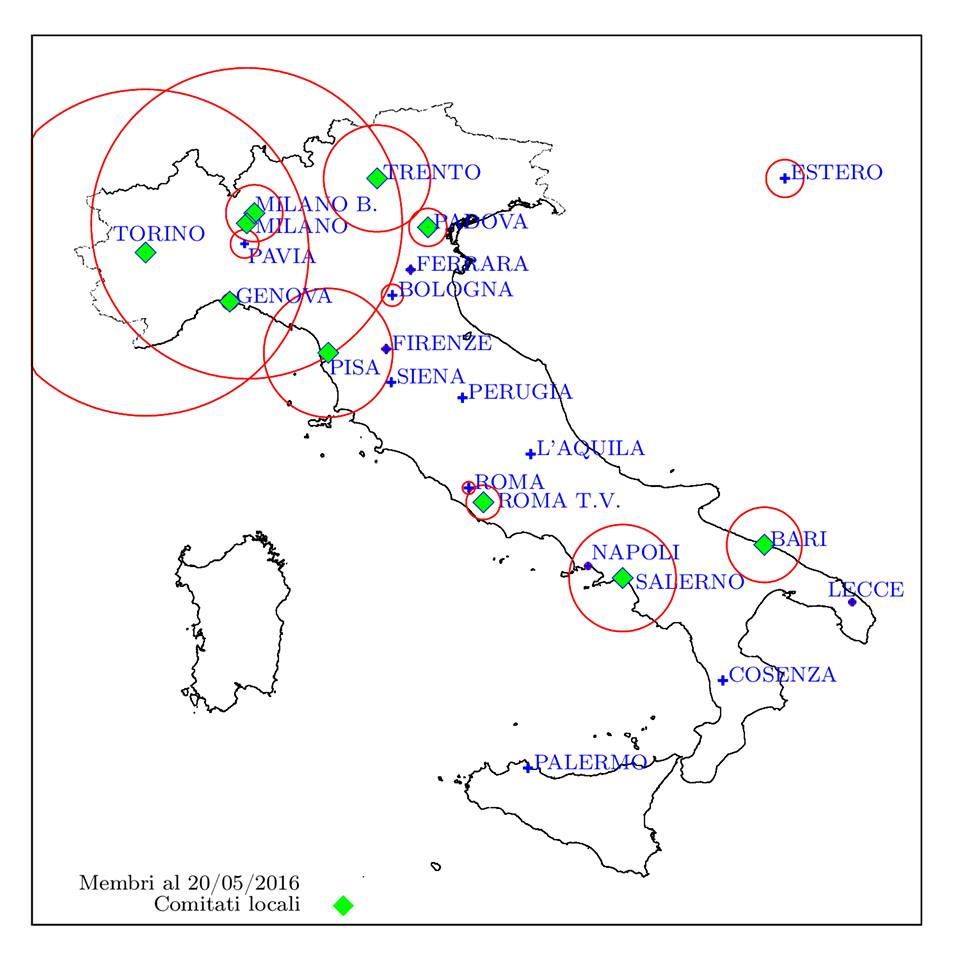
\includegraphics[scale=0.23]{images/provenienza.png}
\end{figure}
\end{frame}
\subsection{Comitati Locali}
\begin{frame}{Comitati Locali}
\begin{figure}
\begin{block}{\centering \textbf{Comitati Locali Presenti}}
\begin{itemize}
\begin{columns}
\begin{column}{0.3\textwidth}
\item Torino
\item Milano
\item Pisa
\item Trento
\item Bari
\item Salerno
\end{column}
\begin{column}{0.2\textwidth}
\item Genova
\item Milano Bicocca
\item Padova
\item Roma [soon...]
\item Pavia [soon...]
\item Firenze [soon...]
\end{column}
\end{columns}
\end{itemize}
\end{block}
\end{figure}
\end{frame}
\section{Divulgazione}
\begin{frame}
\begin{block}{\centering{\fontsize{30}{100}\selectfont DIVULGAZIONE}}
\end{block}
\end{frame} 
\begin{frame}{Attività di Divulgazione}
\begin{figure}
\begin{block}{\centering \textbf{Attività Comitati Locali}}
\begin{itemize}
\item \textbf{{Bari}} - International Year of Light School Day
\item \textbf{{Torino}} - Particle Beers
\item \textbf{{Pisa}} - Matter of Physics
\item \textbf{{Torino}} - AstroWine [soon...]
\end{itemize}
\end{block}
\begin{block}{\centering \textbf{Divulgazione nelle scuole}}
\begin{itemize}
\item \textbf{Chi}: 5 relatori - 3° e 4° anno di studi
\item \textbf{Per chi}: 3° 4° 5° anno Licei e Istituti Tecnici
\item \textbf{Dove}:
	\begin{itemize}
	\item Torino
	\item Moncalieri (TO)
	\item Gavirate (VA)
	\item Saronno (VA)
	\end{itemize}
\end{itemize}
\end{block}
\end{figure}
\end{frame}
\subsection{MoP}
\begin{frame}{International Year of Light School Day}
\begin{figure}
\begin{columns}
\begin{column}{0.5\textwidth}
\vspace{1mm}
\centering 
\textbf{Bari}, 10 novembre 2015 \\ \vspace{0.5cm}
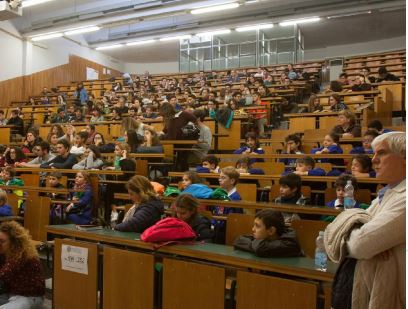
\includegraphics[width=6cm]{images/SD22.jpg}
\end{column}
\begin{column}{0.5\textwidth}\centering
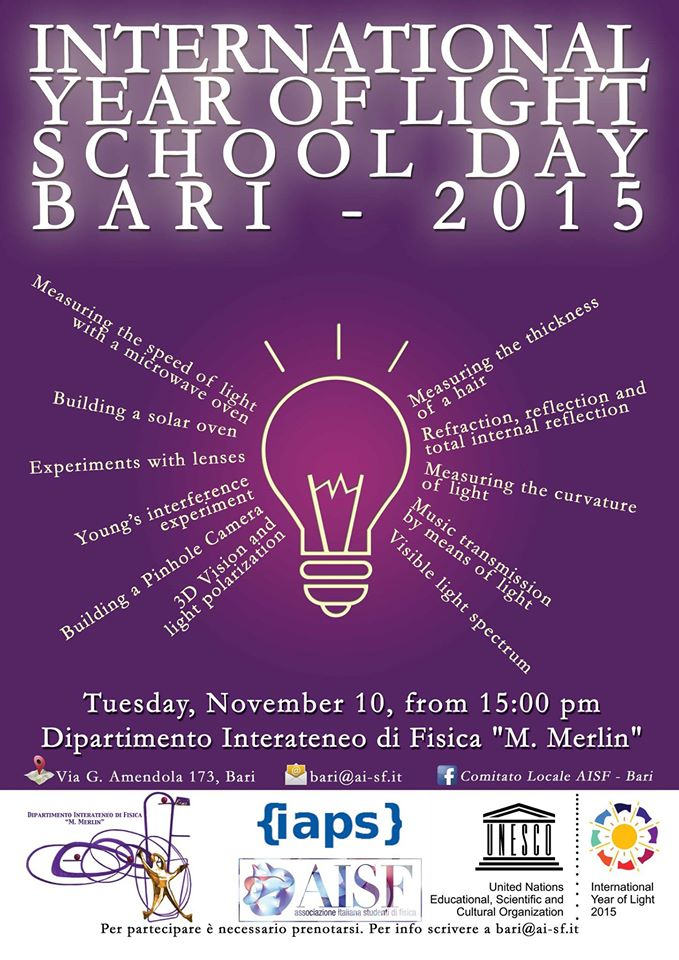
\includegraphics[width=4cm]{images/SD1.jpg}
\end{column}
\end{columns}
\end{figure}
\end{frame}
\subsection{PB}
\begin{frame}{Particle Beers}
\begin{figure}
\begin{columns}
\begin{column}{0.5\textwidth}
\vspace{1mm}
\centering 
\textbf{Torino}, 20 gennaio 2016 \\ \vspace{0.5cm}
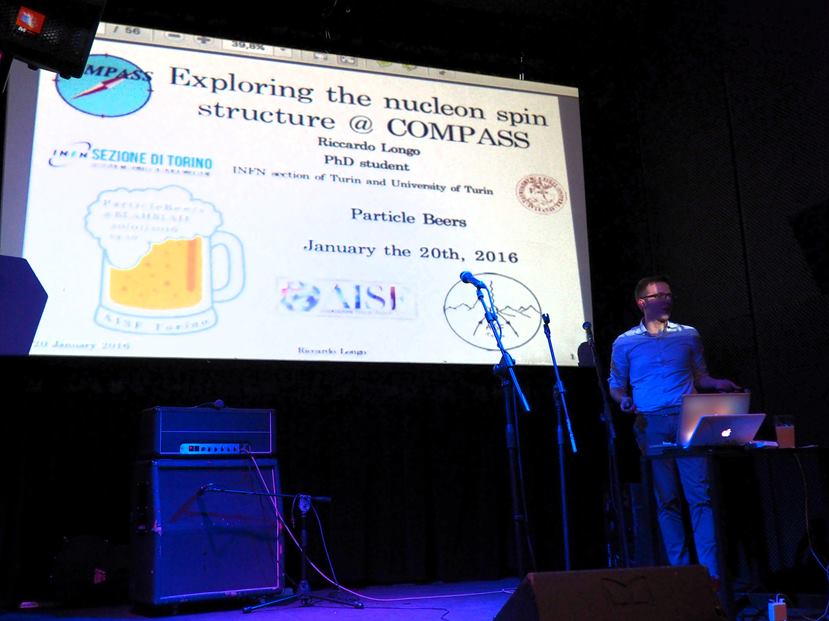
\includegraphics[width=6cm]{images/PB2.jpg}
\end{column}
\begin{column}{0.5\textwidth}\centering
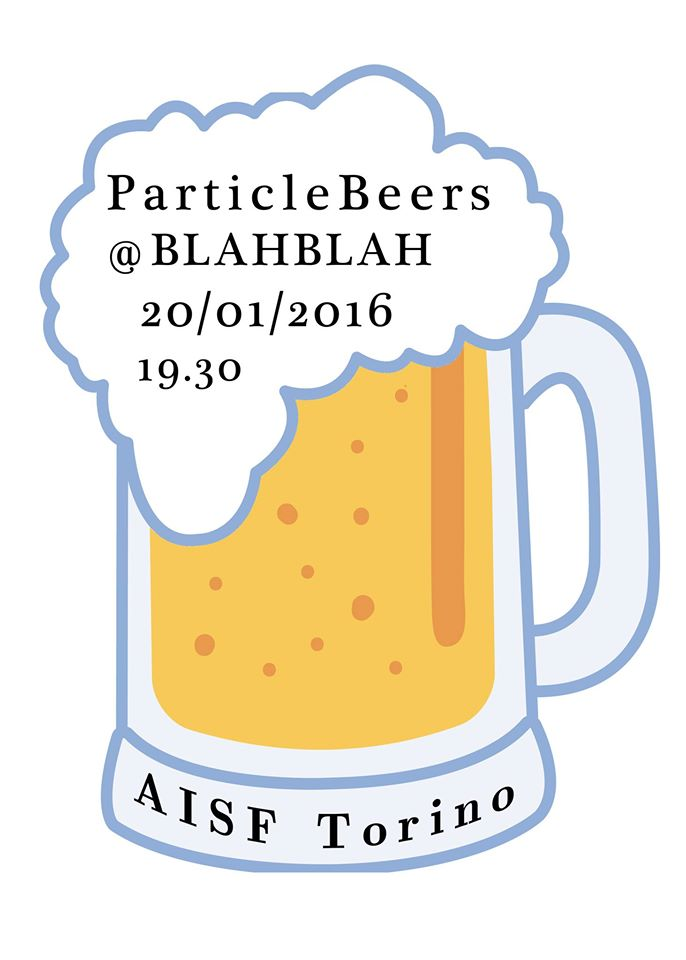
\includegraphics[width=4cm]{images/PB1.jpg}
\end{column}
\end{columns}
\end{figure}
\end{frame}
\subsection{MoP}
\begin{frame}{Matter of Physics}
\begin{figure}
\begin{columns}
\begin{column}{0.5\textwidth}
\vspace{1mm}
\centering 
\textbf{Pisa}, 17 maggio 2016 \\ \vspace{0.5cm}
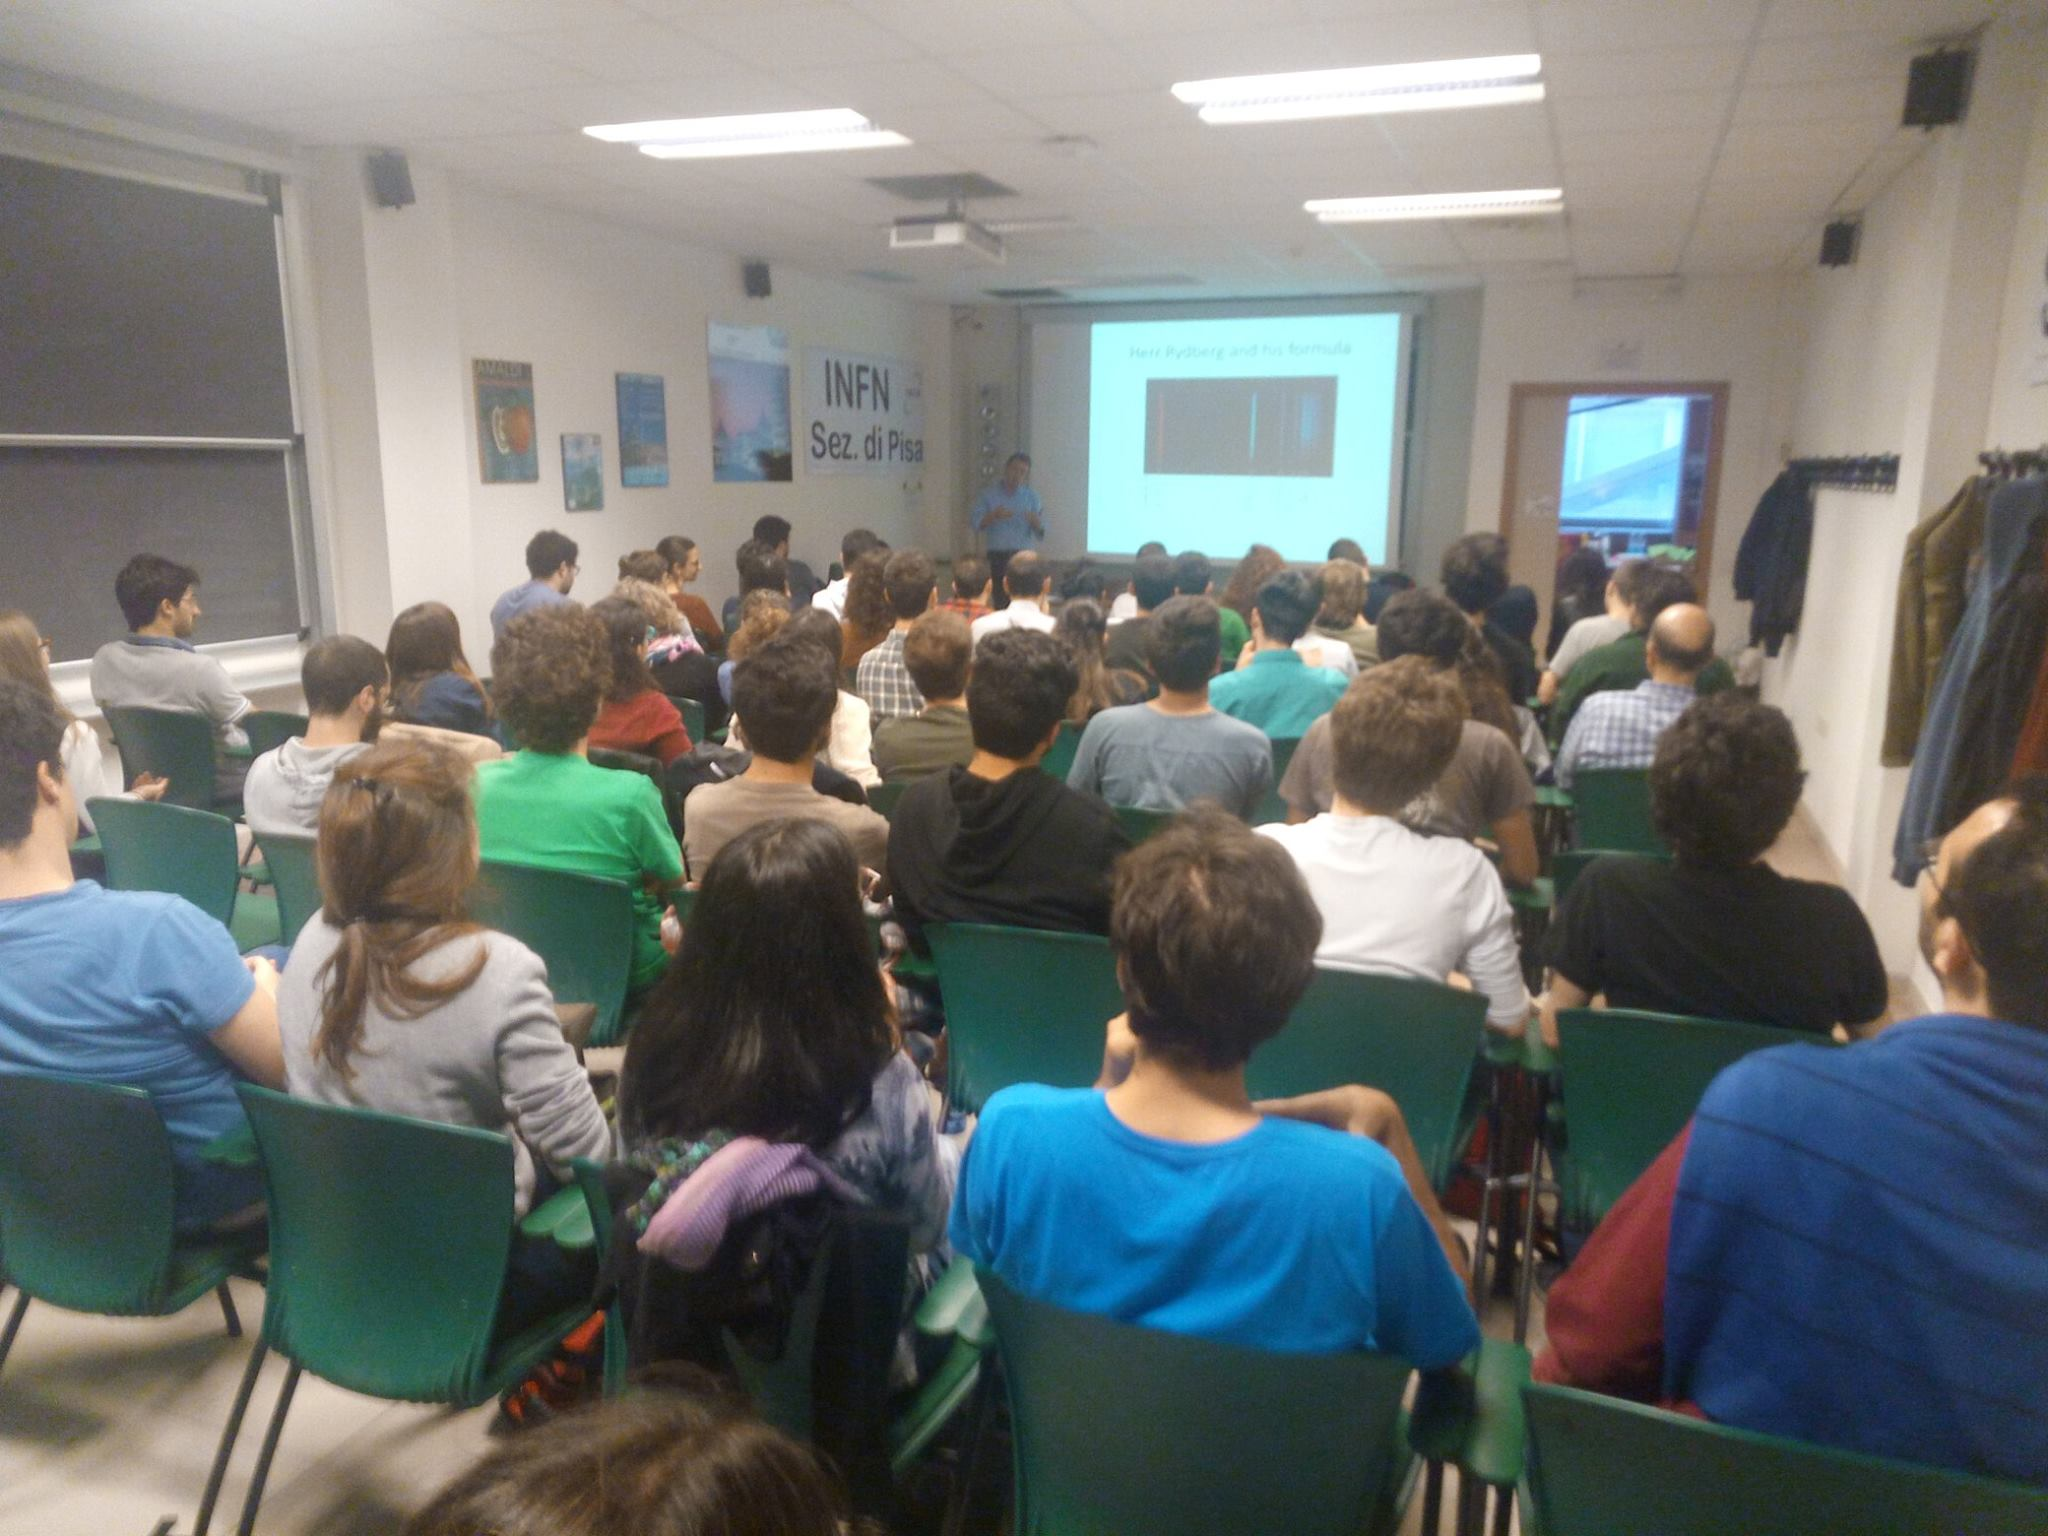
\includegraphics[width=6cm]{images/MoP2.jpg}
\end{column}
\begin{column}{0.5\textwidth}\centering
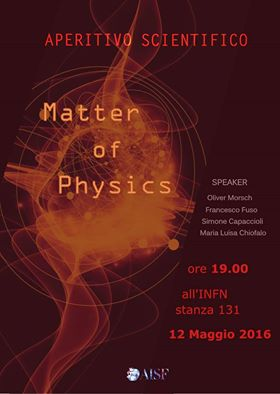
\includegraphics[width=4cm]{images/MoP1.jpg}
\end{column}
\end{columns}
\end{figure}
\end{frame}


\section{Eventi}
\begin{frame}
\begin{block}{\centering{\fontsize{30}{100}\selectfont EVENTI}}
\end{block}
\end{frame} 

\begin{frame}{Eventi AISF - IAPS}
\begin{figure}
\begin{block}{\centering \textbf{Eventi Nazionali}}
\begin{itemize}
\item \textbf{{Milano}} - Visita al Laboratorio Acceleratori e Superconduttività Applicata
\item \textbf{{Torino}} - Conferenza Italiana Studenti di Fisica 2016
\item \textbf{{Pisa}} - Visita a EGO-VIRGO [soon...]
\item \textbf{{Milano}} - Visita all' Osservatorio Astronomico "G.V. Schiaparelli" [31 maggio 2016] 
\end{itemize}
\end{block}
\begin{block}{\centering \textbf{Eventi Internazionali}}
\begin{itemize}
\item \textbf{Pisa}: Lights of Tuscany
\item \textbf{Gran Sasso} : Particle \& Astroparticle Physics Programme
\item \textbf{Torino}: International Conference of Physics Students
\item \textbf{Altri Eventi IAPS}:
	\begin{itemize}
	\item IAPS2Cern
	\item IAPS4Fusion
	\item PLANCKS
	\end{itemize}
\end{itemize}
\end{block}
\end{figure}
\end{frame}


\subsection{CISF2016}
\begin{frame}{Conferenza Italiana Studenti di Fisica}
\begin{figure}
\begin{columns}
\begin{column}{0.5\textwidth}
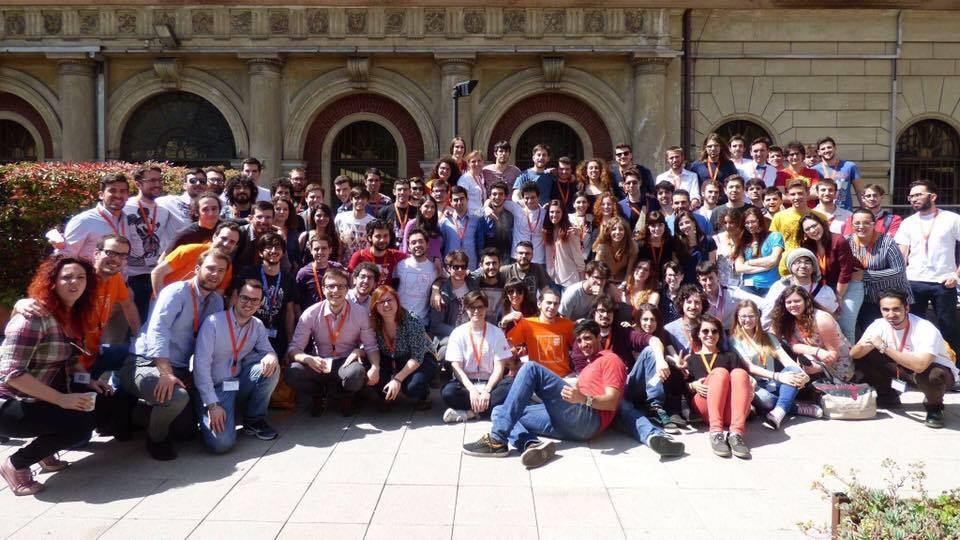
\includegraphics[width=5.7cm]{images/CISF1.jpg}
\\
\centering \textbf{Torino}, 22-24 aprile 2016
\end{column}
\begin{column}{0.5\textwidth}
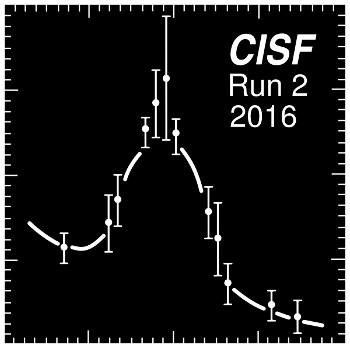
\includegraphics[width=5cm]{images/CISF2.jpg}
\end{column}
\end{columns}
\end{figure}
\end{frame}
\subsection{LASA}
\begin{frame}{Laboratorio Acceleratori e Superconduttività Applicata}
\begin{figure}
\begin{columns}
\begin{column}{0.5\textwidth}
\\
\centering \textbf{Segrate (MI)}, 2 marzo 2016
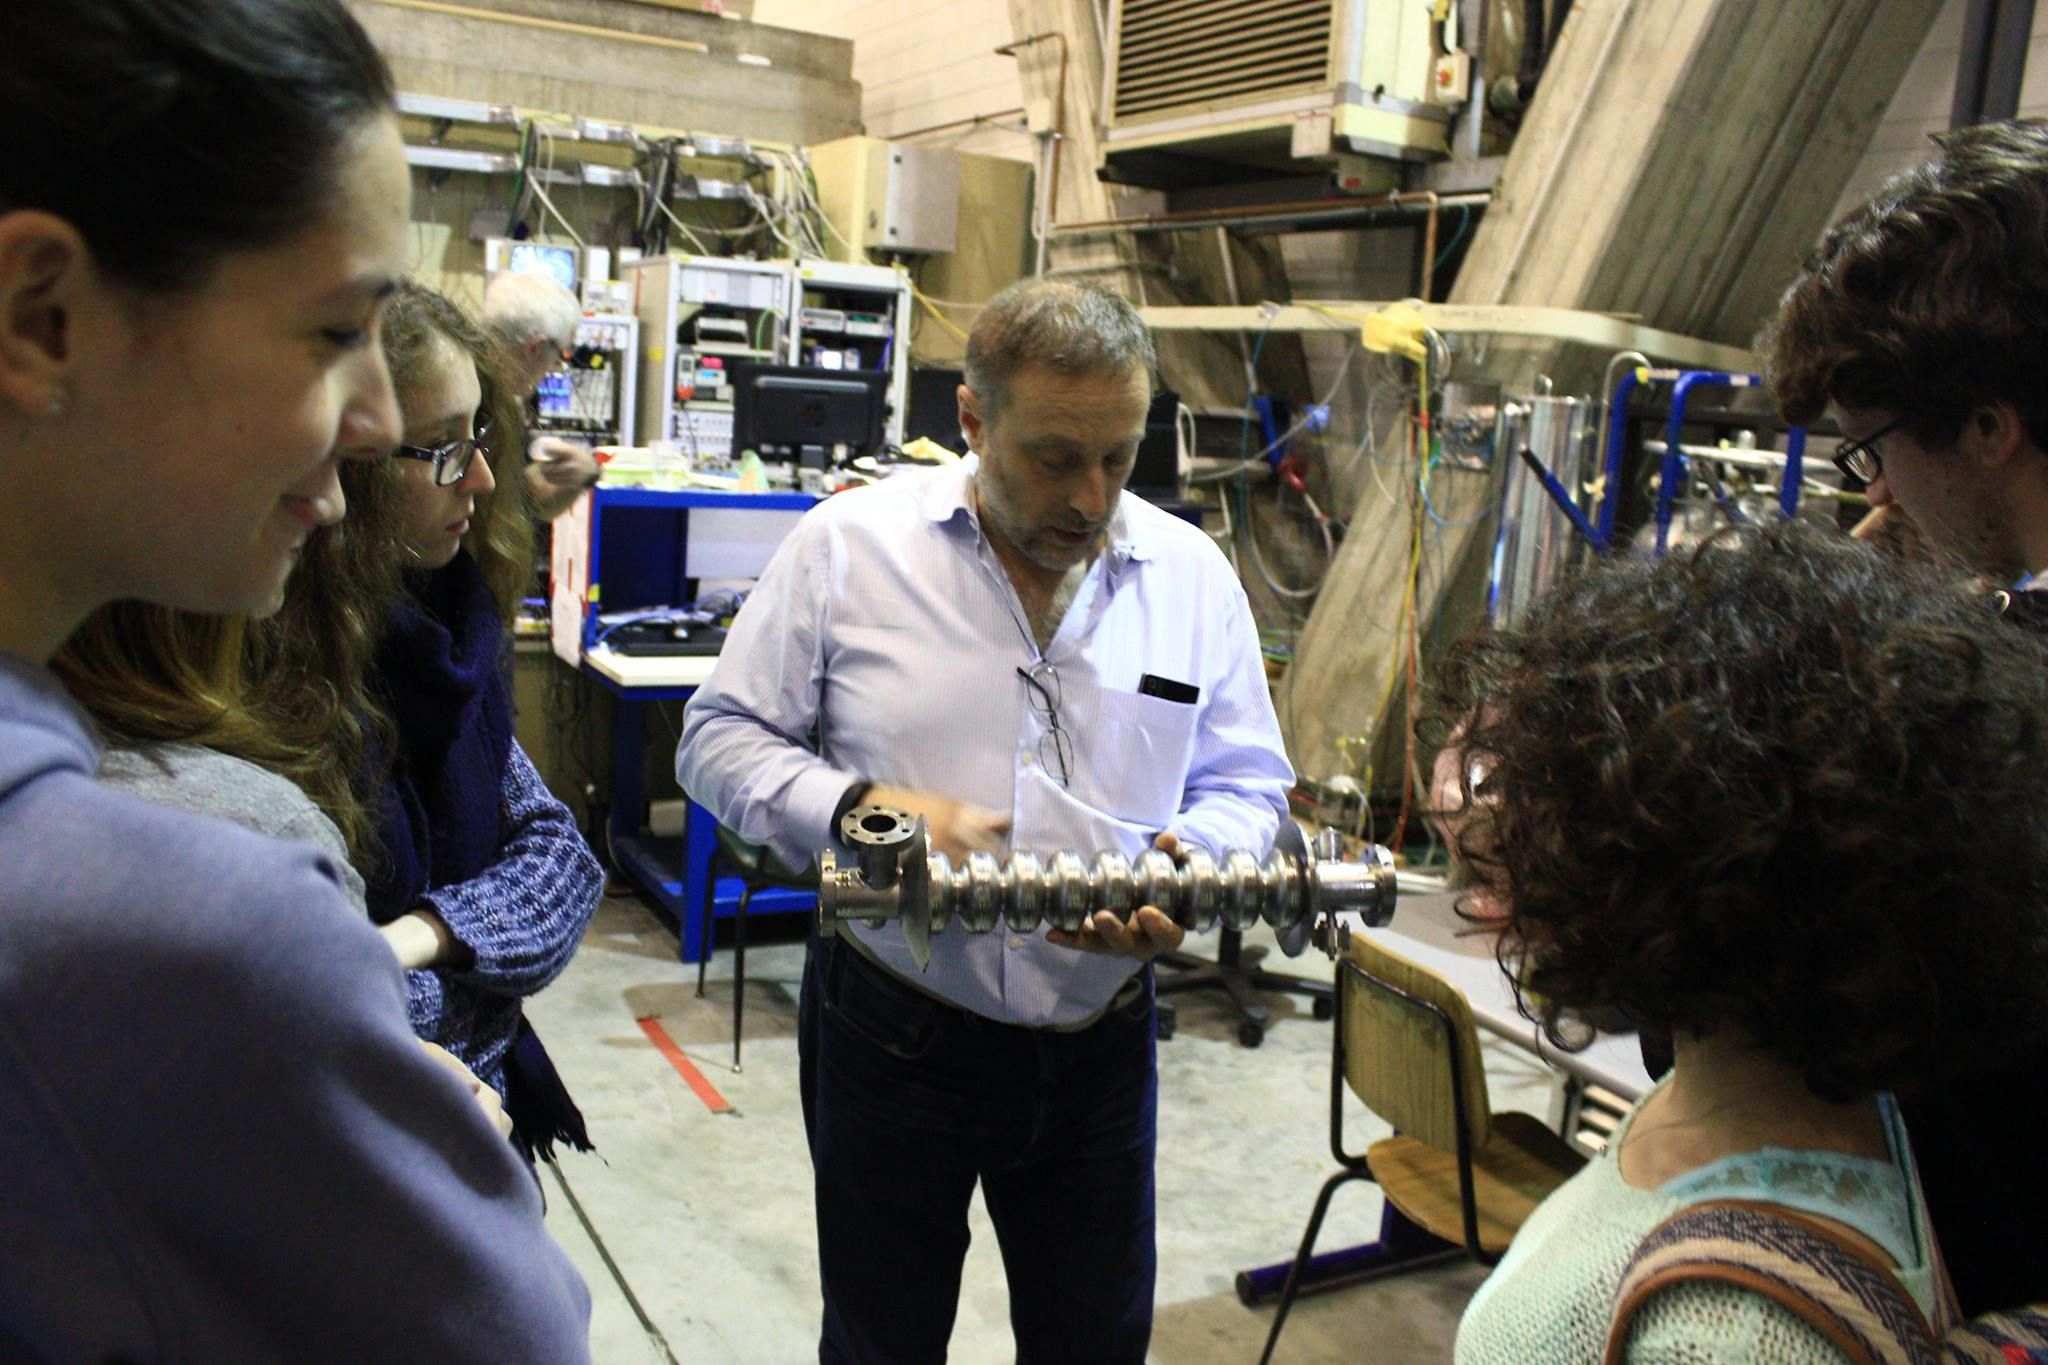
\includegraphics[width=5.7cm]{images/LASA1.jpg}

\end{column}
\begin{column}{0.5\textwidth}
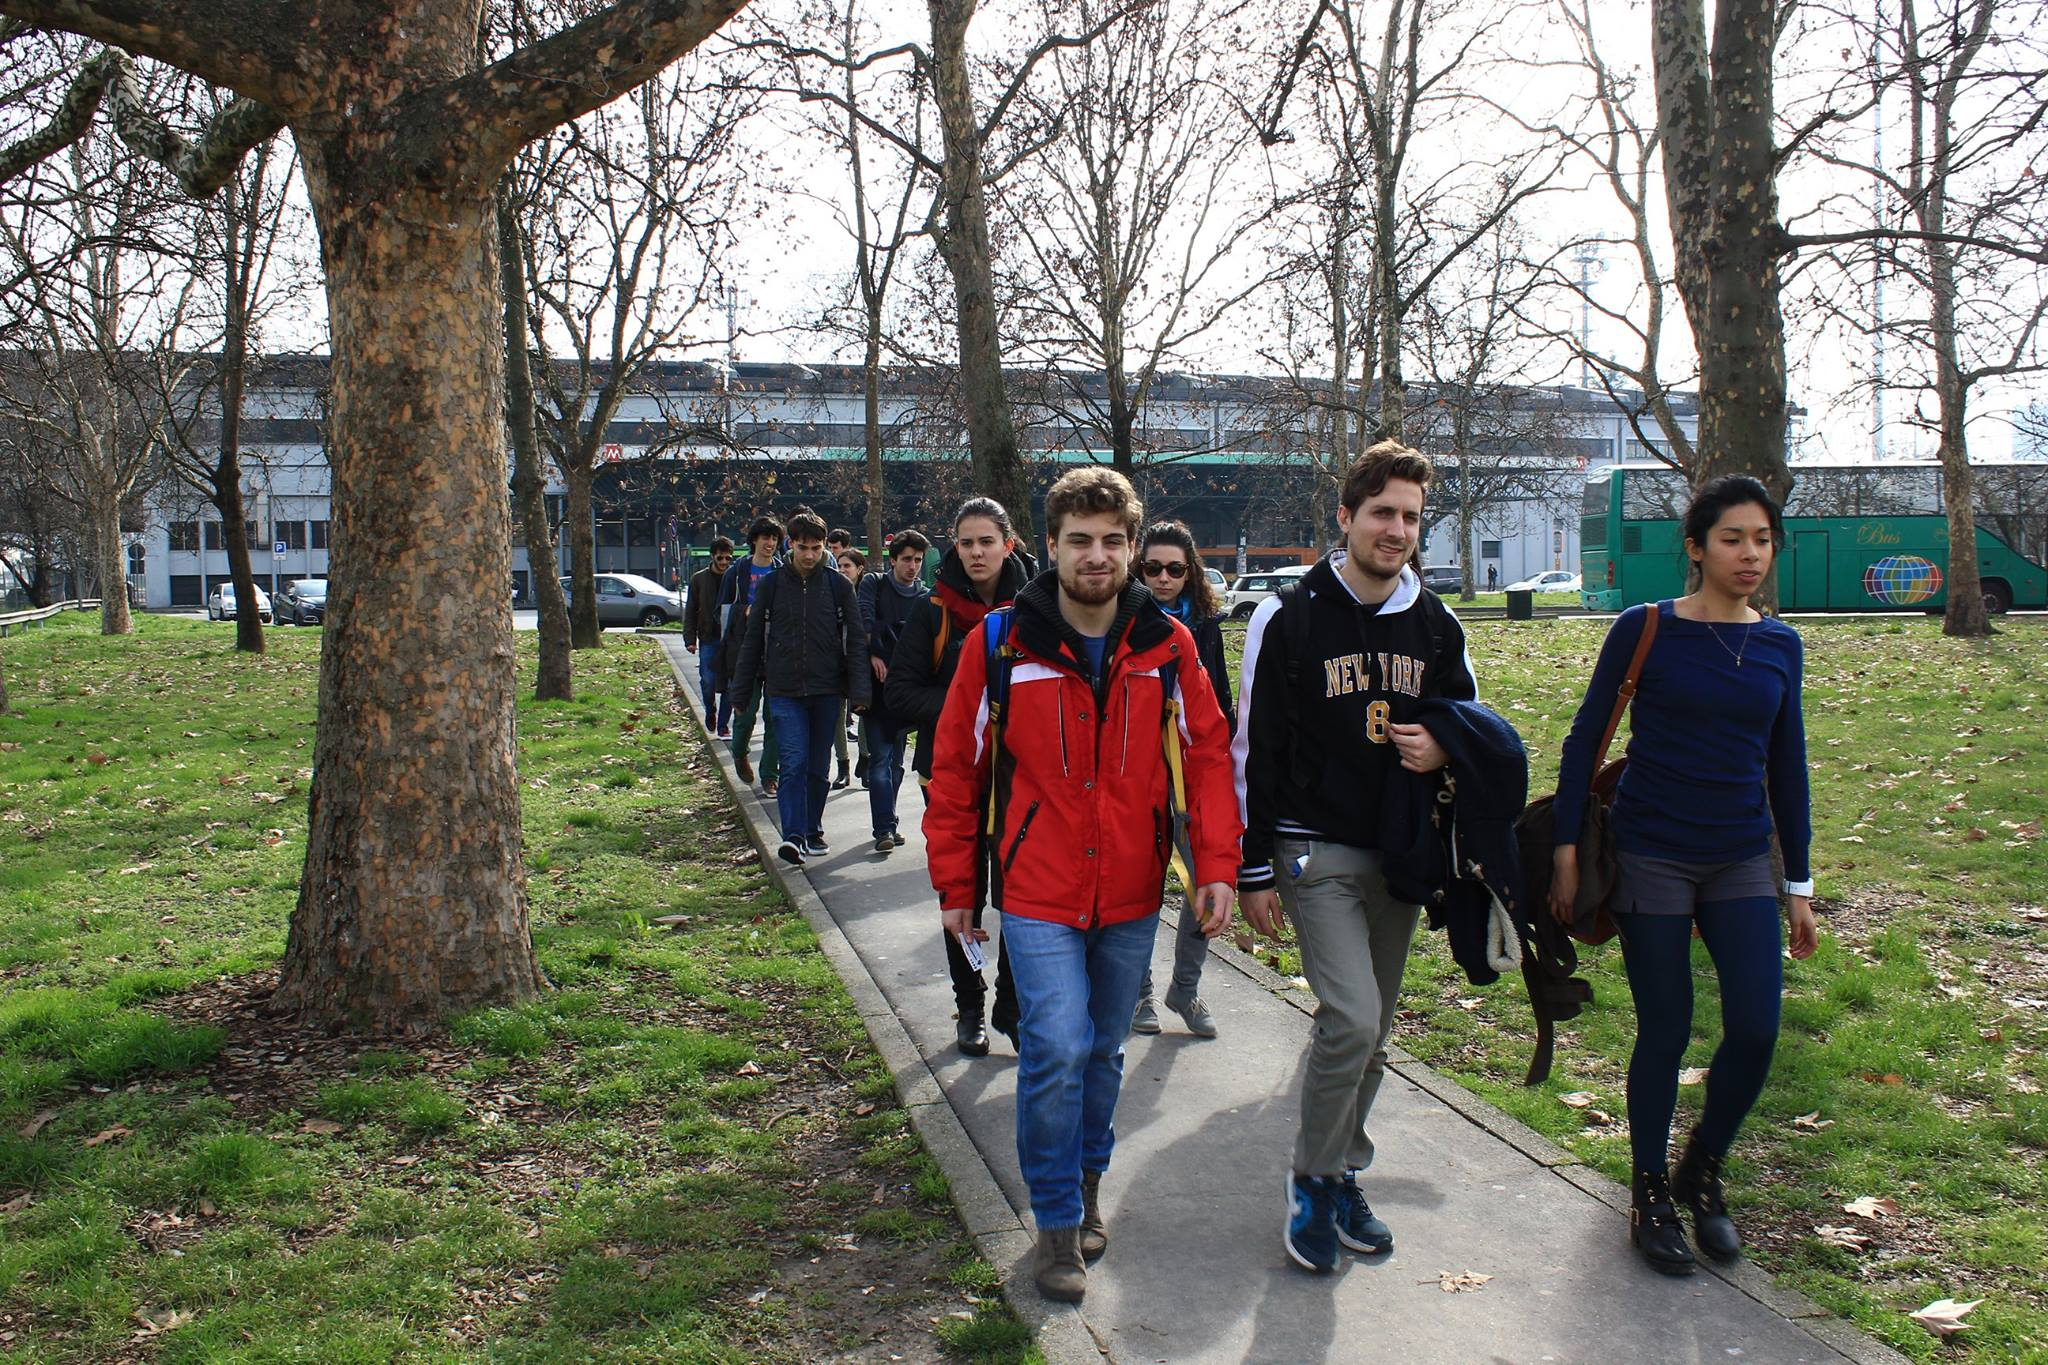
\includegraphics[width=5cm]{images/LASA2.jpg}
\end{column}
\end{columns}
\end{figure}
\end{frame}
\subsection{LoT}
\begin{frame}{Lights of Tuscany}
\begin{figure}
\begin{columns}
\begin{column}{0.5\textwidth}
\vspace{1mm}
\centering 
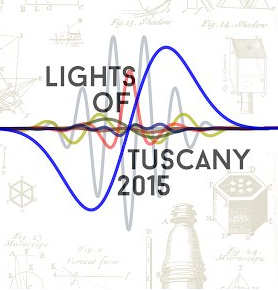
\includegraphics[width=2cm]{images/LoT1.png}\\
\textbf{Toscana}, 17-21 dicembre 2015 \\ \vspace{0.5cm}
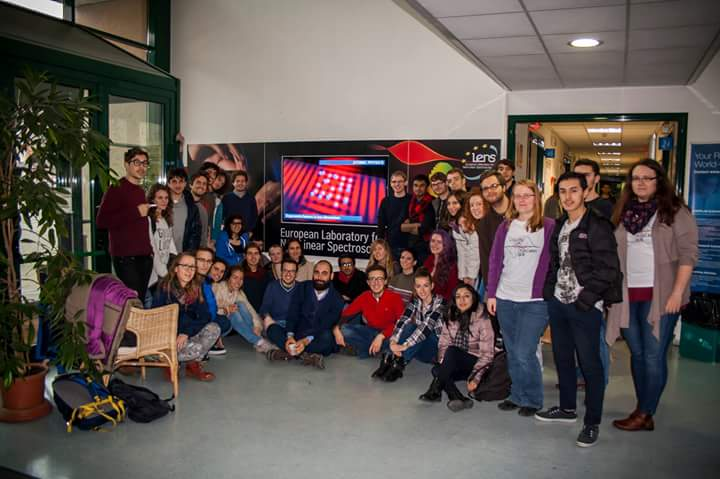
\includegraphics[width=6cm]{images/LoT6.jpg}
\end{column}
\begin{column}{0.5\textwidth}\centering
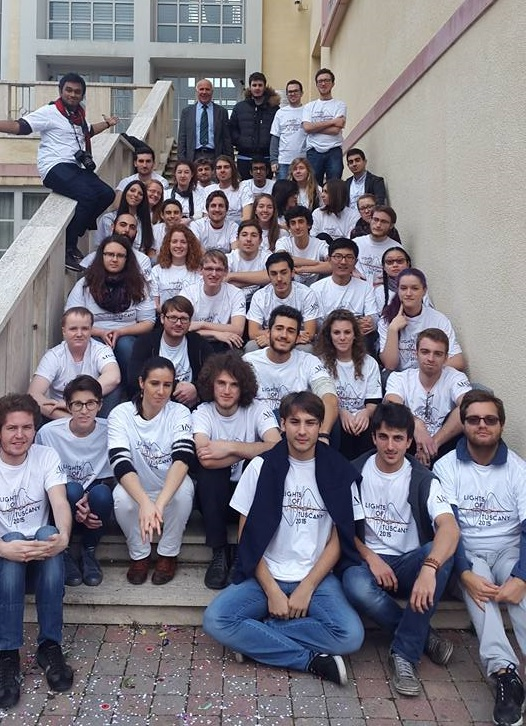
\includegraphics[width=4cm]{images/LoT2.jpg}
\end{column}
\end{columns}
\end{figure}
\end{frame}
\begin{frame}{}
\vspace{2mm}
\begin{figure}
\begin{columns}
\begin{column}{0.5\textwidth}
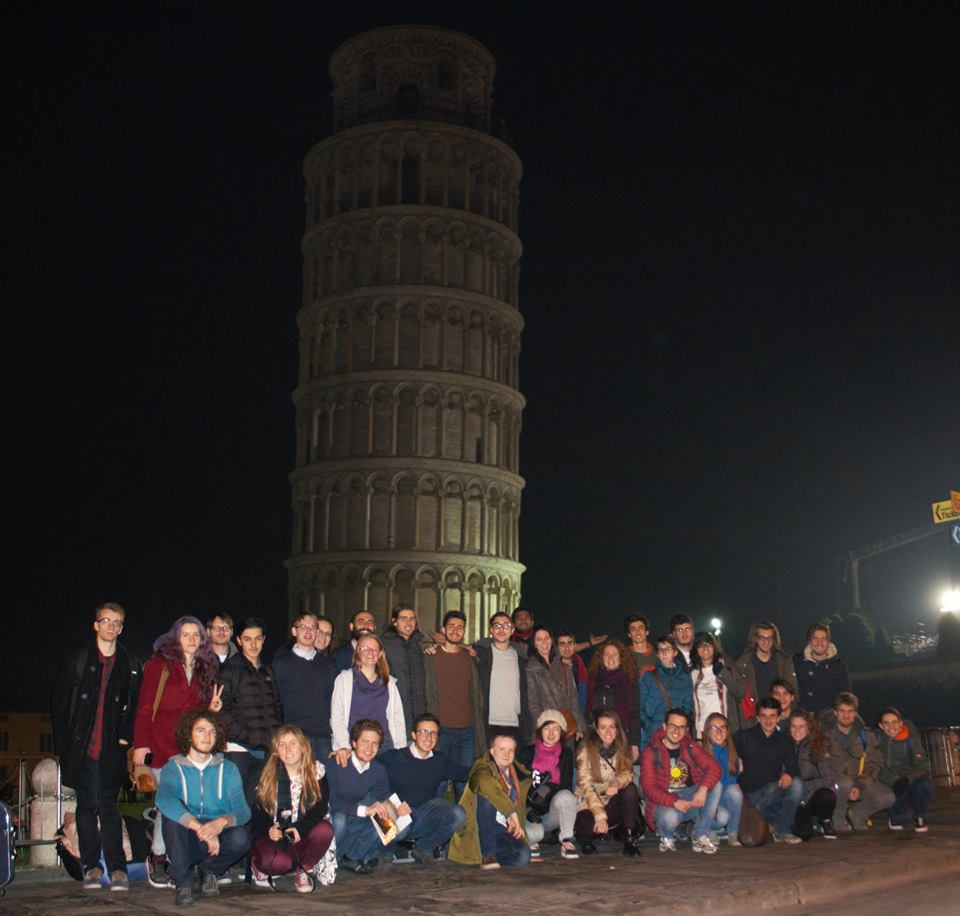
\includegraphics[width=5.5cm]{images/LoT4.jpg} \\
\end{column}
\vspace{2mm}
\begin{column}{0.5\textwidth}
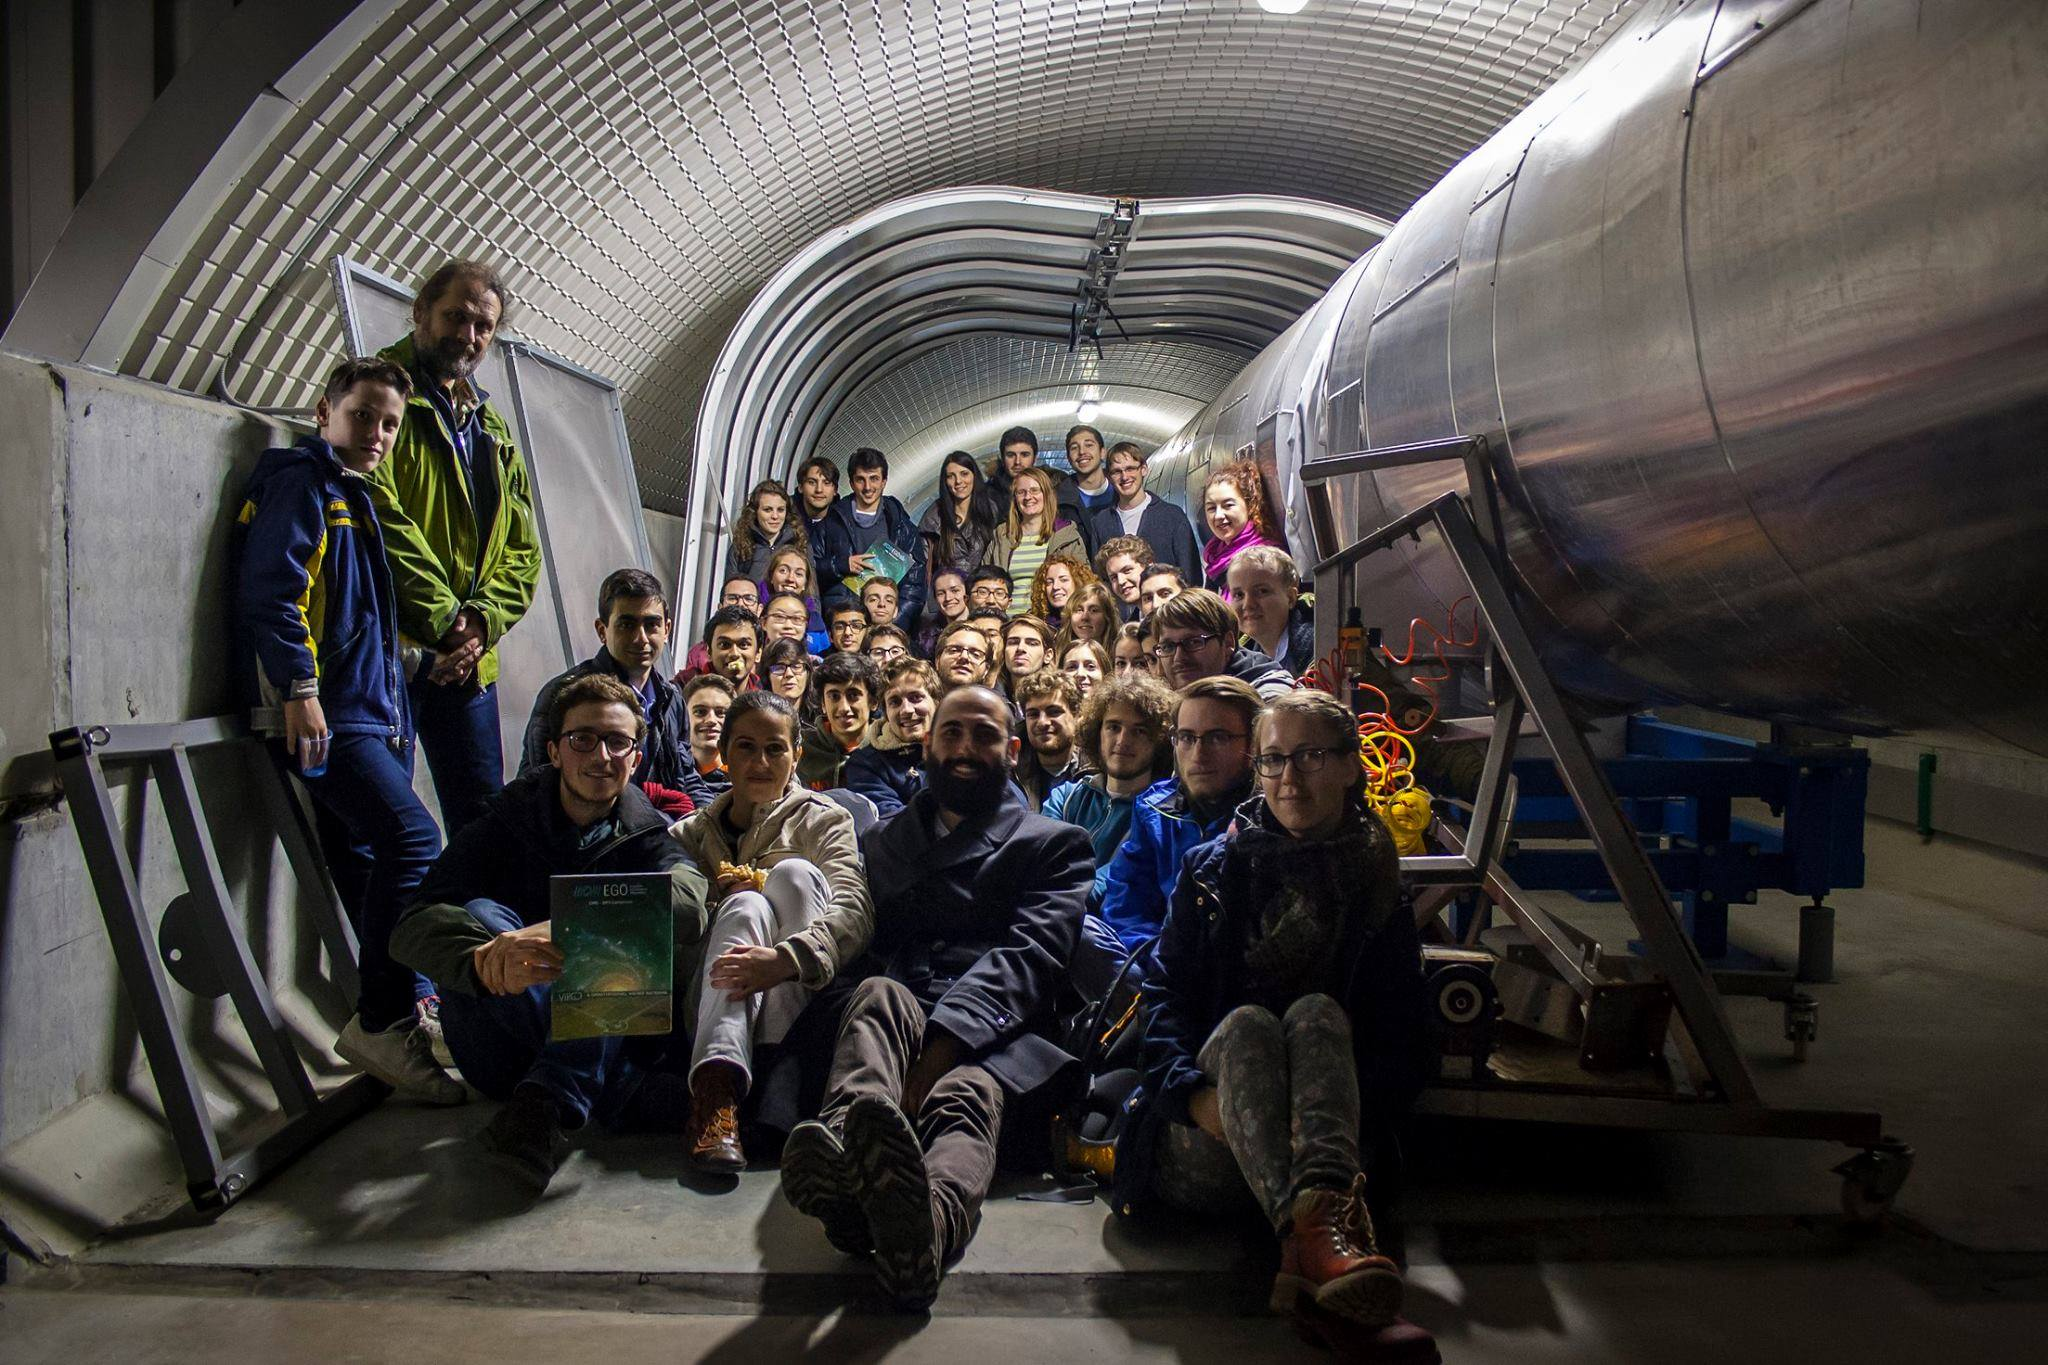
\includegraphics[width=5.5cm]{images/LoT5.jpg}
\\ \vspace{0.2cm}
\centering
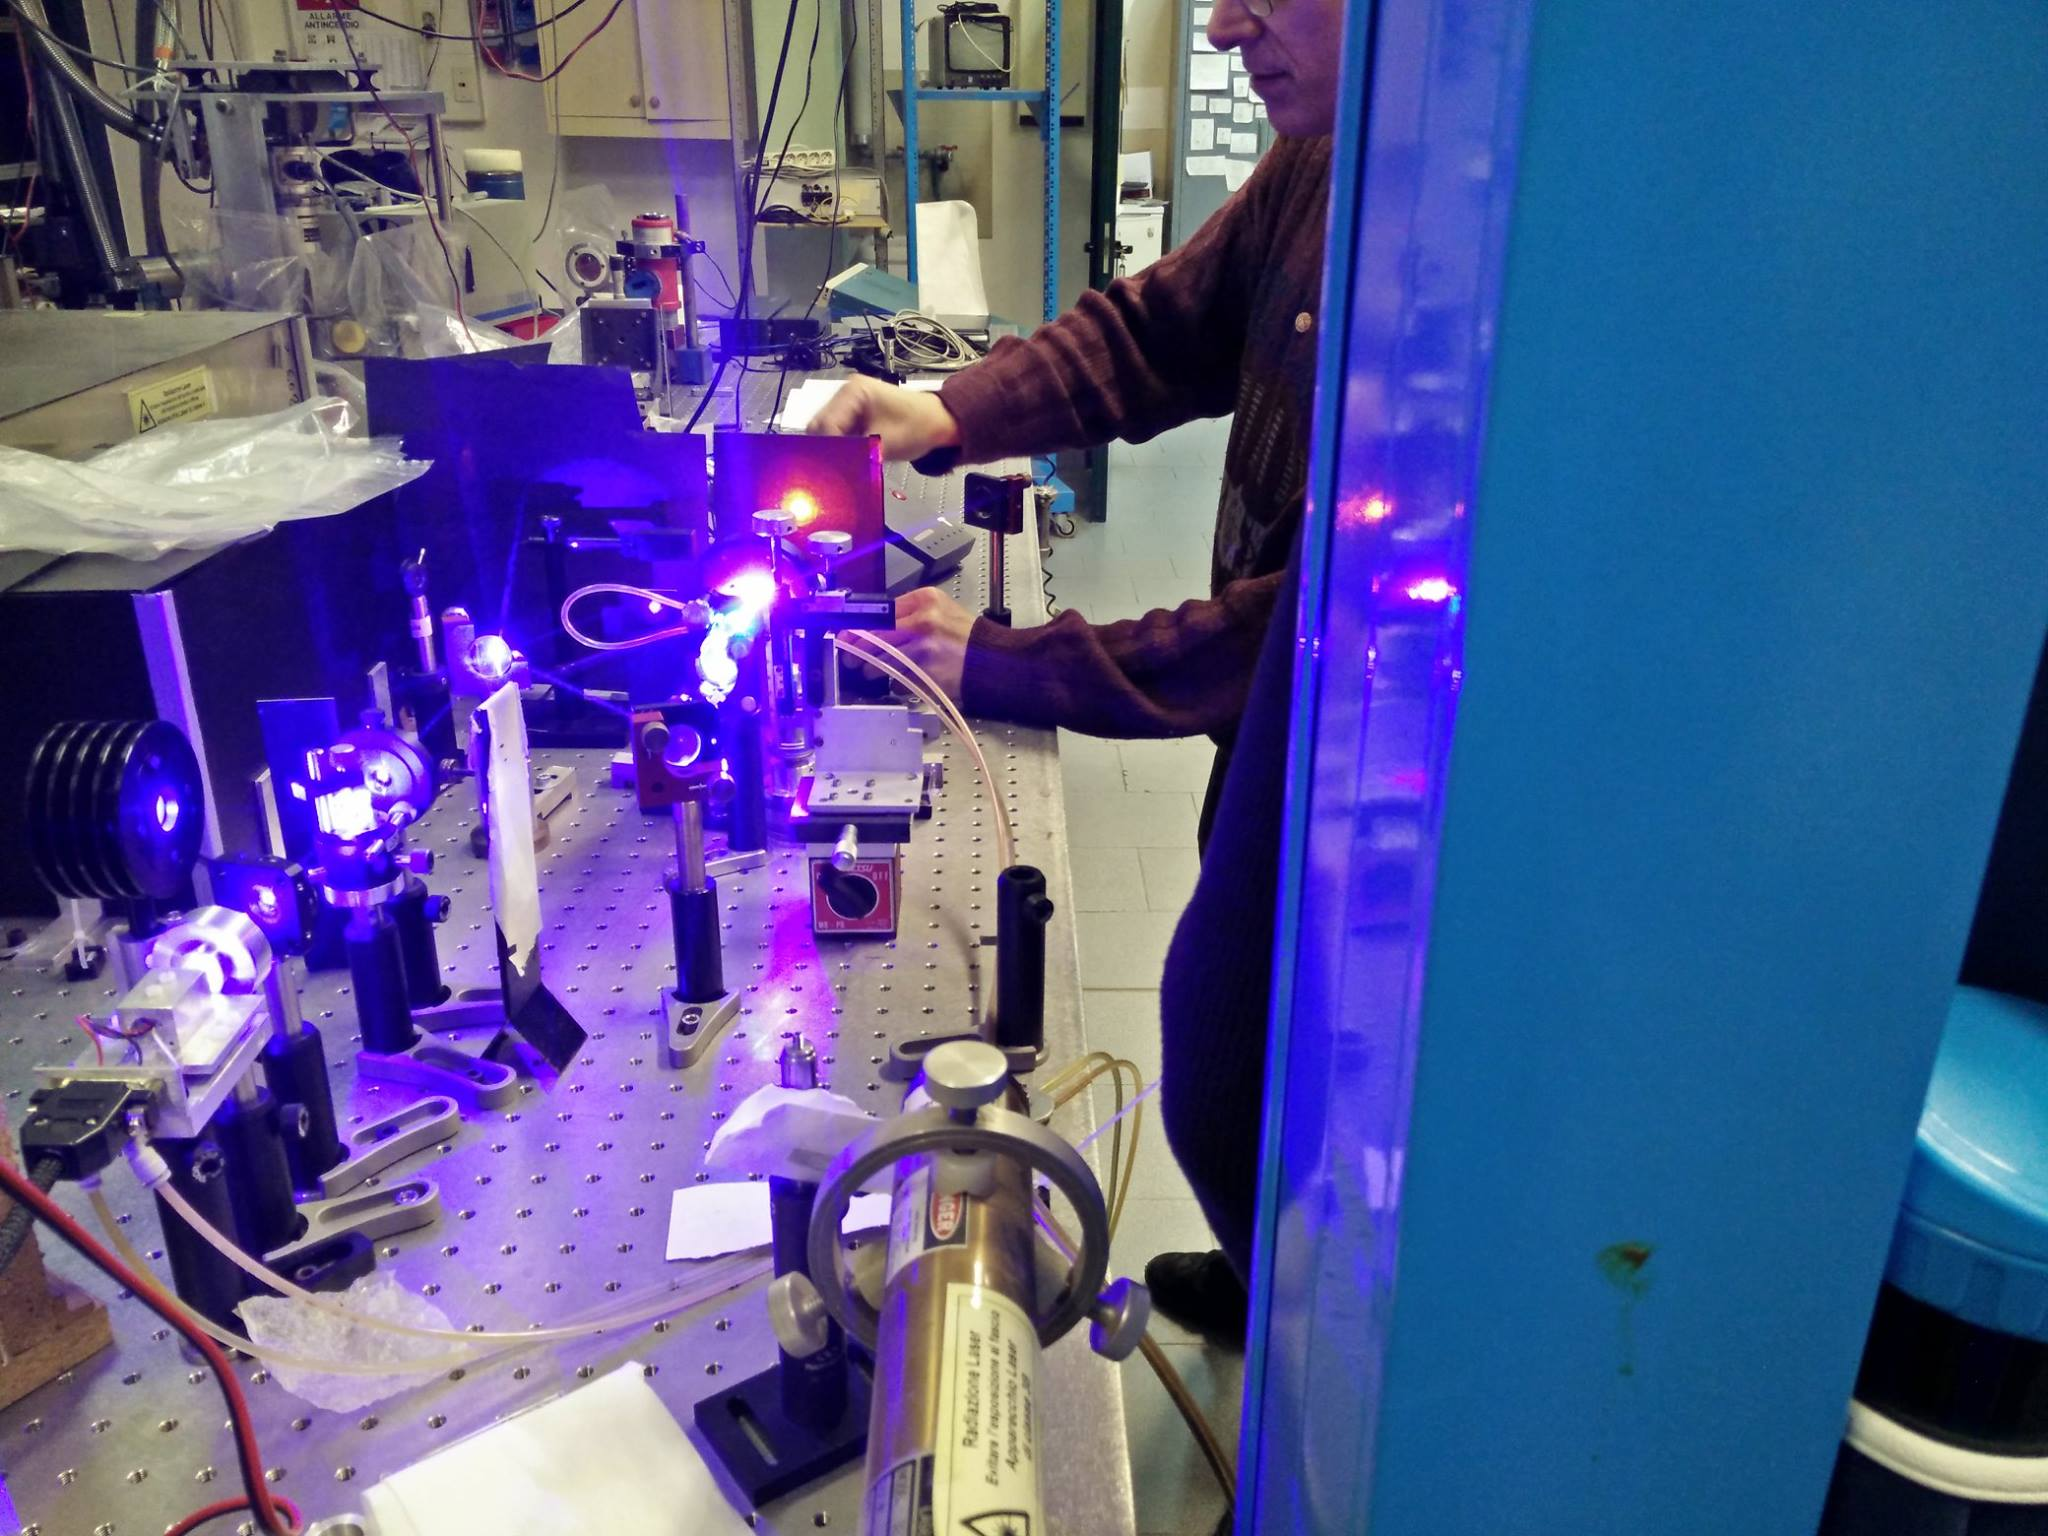
\includegraphics[width=4.3cm]{images/LoT3.jpg}
\end{column}
\end{columns}
\end{figure}
\end{frame}
\subsection{APAP}
\begin{frame}{Particle \& Astroparticle Physics Programme}
\begin{figure}

\centering 
\includegraphics[width=4cm]{images/IAPSGS.png} \\ \textbf{Frascati-GranSasso}, fine settembre 2016 \vspace{1mm}
\begin{columns}
\begin{column}{0.5\textwidth}
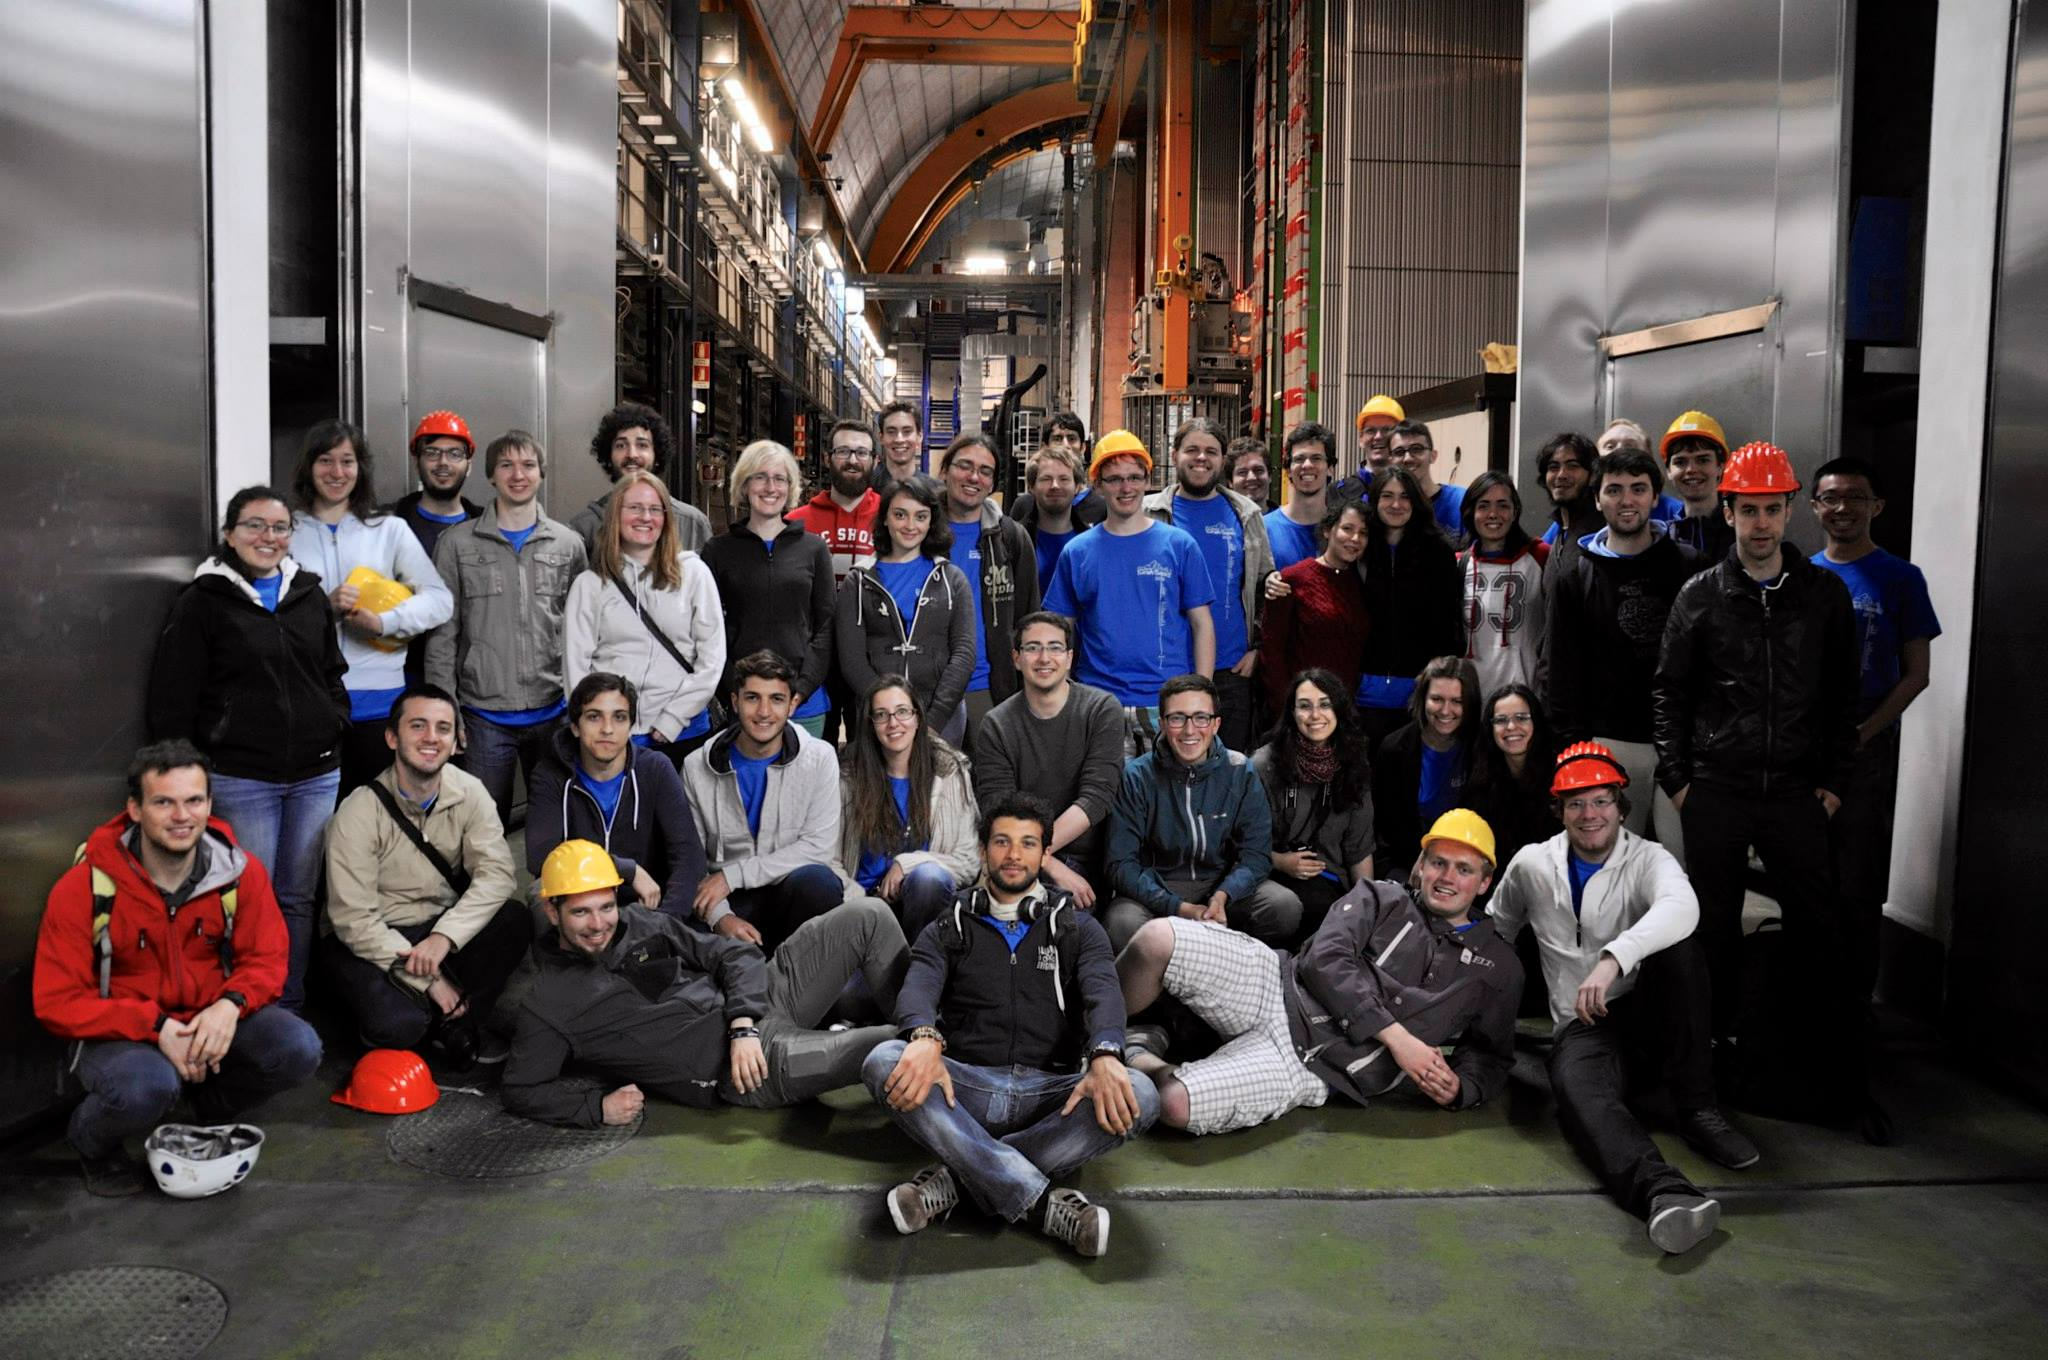
\includegraphics[width=5.55cm]{images/GRANSASSO.jpg} \\
\end{column}
\begin{column}{0.5\textwidth}
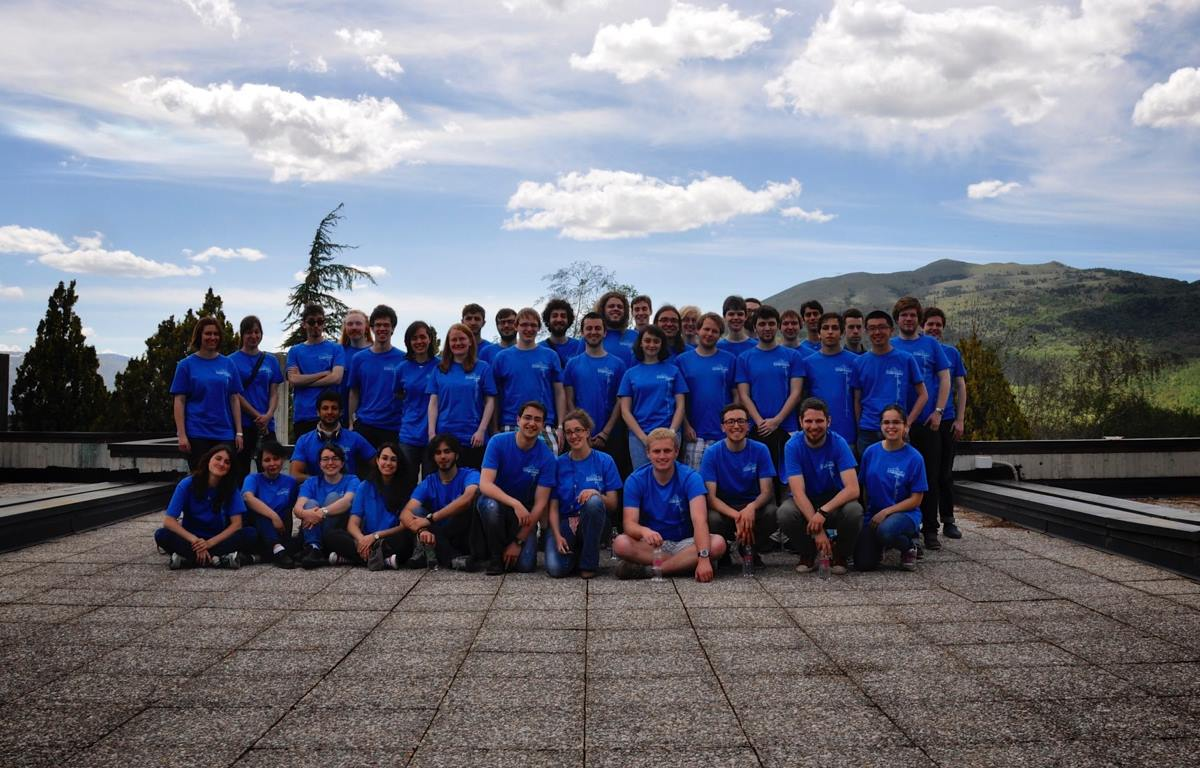
\includegraphics[width=5.7cm]{images/GS.jpg}
\end{column}
\end{columns}
\end{figure}
\end{frame}
\subsection{Altri Eventi}
\begin{frame}{Eventi IAPS}
\begin{block}{\centering \textbf{Altri Eventi}}
\vspace{3mm} \centering
 \includegraphics[width=4cm]{images/IAPS4FUSION.png}
 
\includegraphics[width=4cm]{images/PLANCKS.png} \\
 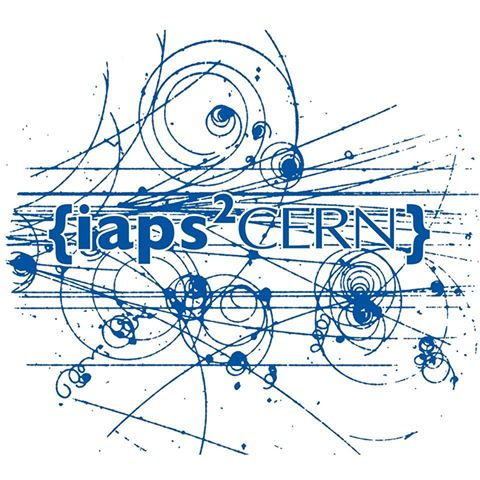
\includegraphics[width=3.2cm]{images/IAPS2CERN.jpg}
\end{block}
\end{frame}
\subsection{ICPS2017}
\begin{frame}{International Conference of Physics Students}
\begin{figure}

 
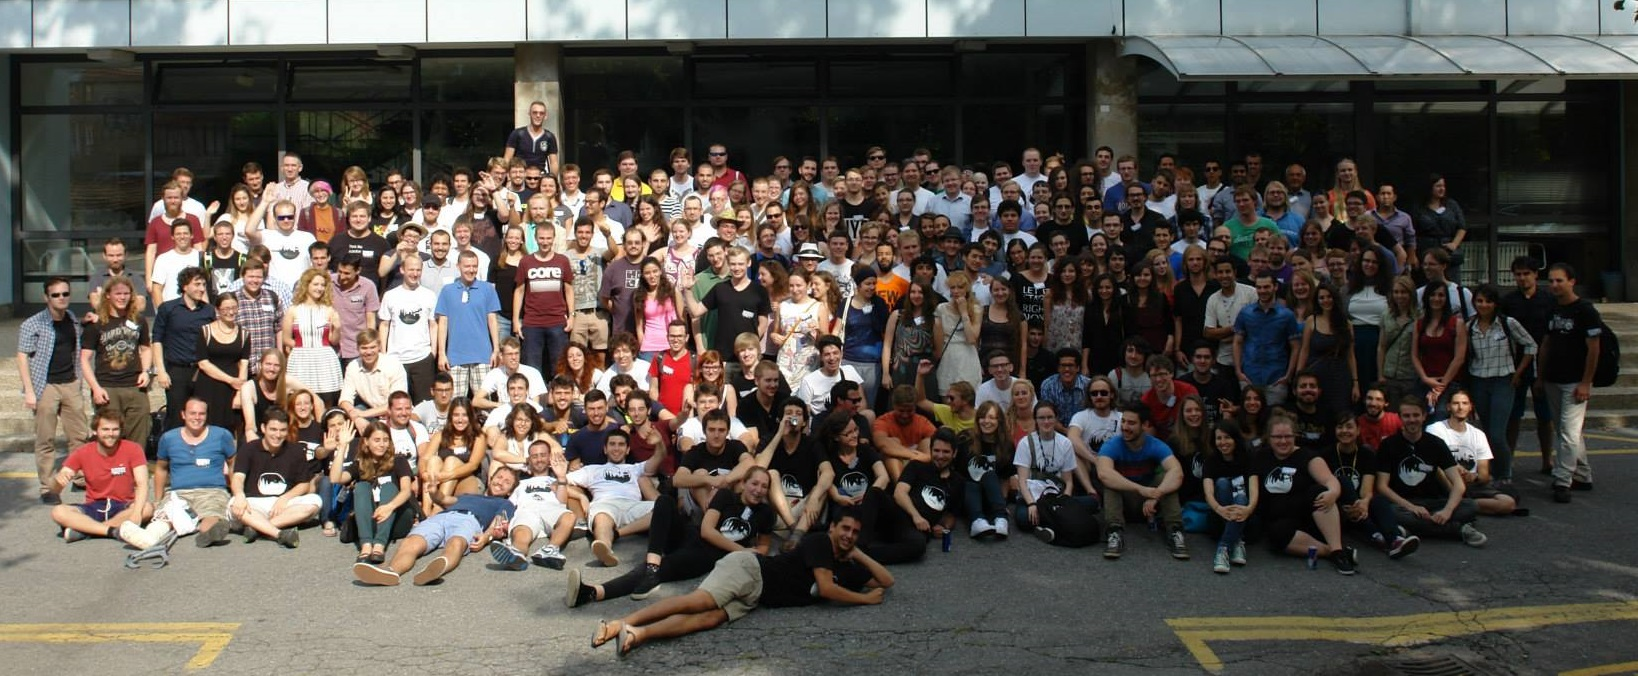
\includegraphics[width=10cm]{images/ICPS.jpg} \\
\begin{columns}
\begin{column}{0.3\textwidth}

\includegraphics[width=4cm]{images/ICPS2017.png}
\end{column}
\begin{column}{0.7\textwidth}
\Huge{\textbf{Torino}, 7-14 agosto 2017} \\
\end{column}
\end{columns}
\end{figure}
\end{frame}
\section{FERMI}
\begin{frame}{Progetto FERMI (Formazione E Ricerca Menti Italiane)}
\begin{figure}
\begin{block}{\centering \textbf{Che cos'è}}
\begin{itemize}
\item Costruzione Database Tirocini e Summer School
\item Recensione Tirocini e Summer School
\item Nuova legislazione per possibilità di Tirocini in Italia
\end{itemize}
\end{block}
\begin{block}{\centering \textbf{Stato Attuale}}
\begin{itemize}
\item 50+ tirocini e Summer School (circa metà pagati) 
\item Mozione votata all'unanimità al CNSU ora da proporre al governo
\item Link mozione: \href{http://www.cnsu.miur.it/argomenti/documentazione/mozioni/2016/mo_2016_03_03_005.aspx}{http://goo.gl/wFAVkq}
\end{itemize}
\end{block}
\end{figure}
\end{frame}


\section{Iscrizioni \& Contatti}
\begin{frame}{Iscrizioni \& Contatti}
\begin{figure}
\begin{block}{\centering \textbf{Iscrizioni}}
{\small Tutte le iscrizioni hanno durata annuale e permettono di partecipare ad ogni evento IAPS e AISF. }
\begin{itemize}
\item Studenti di Laurea Triennale o Magistrale : \textbf{5€}
\item Dottorandi : \textbf{10€}
\end{itemize}
\end{block}
\begin{block}{\centering \textbf{Contatti}}
\begin{itemize}
\item Sito web: \href{http://www.ai-sf.it/joomla/it/}{ai-sf.it}
\item Presidente: presidente@ai-sf.it
\item Esecutivo: esecutivo@ai-sf.it
\item Comitato Locale Pisa: pisa@ai-sf.it %modificalo 
\item Facebook Associazione: \href{https://www.facebook.com/ass.it.stud.fis/?fref=ts}{/ass.it.stud.fis} %da modificare
\item Facebook Comitato Locale: \href{https://www.facebook.com/ComitatoLocalePisa/?fref=ts}{/ComitatoLocalePisa} %da modificare
\item Twitter Associazione: \href{https://twitter.com/aisf_fisica}{@aisf\_fisica}
\end{itemize}
\end{block}
\end{figure}
\end{frame}

\end{document}

